\documentclass[12pt]{article}

\usepackage[margin=1in]{geometry}
\usepackage{amsmath,amsthm,amssymb}
\usepackage{mathtools}
\usepackage{mathrsfs}
\usepackage{enumitem}
\usepackage{physics}
\usepackage{empheq}
\usepackage{undertilde}
\usepackage{float}
\usepackage{graphicx}
\graphicspath{ {./images/} }

\usepackage{tikz}
\usetikzlibrary{calc,decorations.markings,patterns}

\newcommand{\magsq}[1]{\big|#1\big|^2}
\newcommand{\avg}[1]{\left<#1\right>}
\newcommand{\fullint}{\int_{-\infty}^\infty}
\newcommand{\fullintd}[1]{\fullint\dd#1\:}
\newcommand{\cint}[2]{\int_{#1}^{#2}}
\newcommand{\cintd}[3]{\cint{#1}{#2}\dd#3\:}

\begin{document}

\title{Final Exam}
\author{Phys 611}
\date{Due: 12 Noon, Thursday, December 8, 2022 \\ (Willamette Hall Basement Box)}
\maketitle

\section*{Problem 1}
In general relativity, a body moving around a black hole moves so as to minimize its ``proper time'' $\tau$ (i.e. the time measured by a clock moving with the body), which is given by
\begin{equation}
    \tau = \frac{1}{c}\int_{t_0}^{t_f}\sqrt{c^2\gamma(r) - \frac{1}{\gamma(r)}\left(\dv{r}{t}\right)^2 - r^2\left(\dv{\phi}{t}\right)^2} \dd t \tag{1.1}\label{eq:1.1}
\end{equation}
where
\begin{equation}
    \gamma(r) \equiv 1 - \frac{2GM}{rc^2} \tag{1.2}\label{eq:1.2}
\end{equation}
Here $M$ is the mass of the black hole, $c$ is the speed of light, $G$ is the gravitational constant, and $(r,\theta,\phi)$ are the usual spherical coordinates. In equation \refeq{eq:1.1}, and throughout this problem, we'll choose our $\theta=0$ axis such that the body's motion lies in the ``equitorial'' (i.e. $\theta=\frac{\pi}{2}$) plane.
\begin{enumerate}[label=(\alph*)]
    \item Determine the equations of motion that follow from minimizing $\tau$.
    \item Show that for $r \gg r_s\equiv\frac{2GM}{c^2}$, these equations reduce to those of the classical Kepler problem (i.e. standard Newtonian gravity). What is the physical significance of $r_s$?
    \item For the full equations derived in (a), find two conserved quantities.
    \item Using these two conserved quantities, find the effective potential for radial motion, and plot it. If there are qualitatively different shapes of this potential for different values of the conserved quantities, plot all qualitatively different cases, and give the values of the conserved quantities that seperate different cases. \\ (Hint: rewrite the equations replacing $t$ derivatives with $\tau$ derivatives.)  
    \item Describe, qualitatively, the different types of motion possible (by way of illustation, for the Kepler problem, the answer to this question would be: ``closed orbits or escape orbits, \underline{except} in the very special case angular momentum $L=0$, in which case some orbits plunge into the center. When $L\neq 0$, no orbits ever reach the center ($r=0$).'')
    \item For what values of the conserved quantities are stable circular orbits possible?
    \item Calculate the frequency of small radial oscillations about a nearly circular oribt as a function of the radius $r$ of that orbit.
    \item Find the angle $\Delta\theta$ between successive perihelions (or, peri-black-hole-ions), and calculate the precession rate $\frac{\Delta\theta}{T}$, where $T$ is the time between successive perihelions. Compare your answer \underline{qunatitatively} with the observed $\frac{\Delta\theta}{T}$ = 43 arc-seconds/century for mercury.
    \item \[\]
    \begin{figure}[H]
        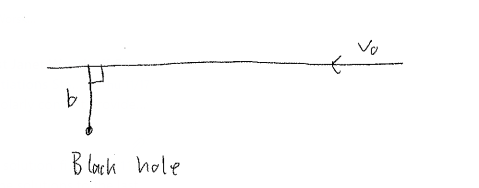
\includegraphics[scale=1]{Problem1}
        \centering
    \end{figure}
    A Projectile is shot towards the black hole from a great distance $r \gg r_s$ away at an initial velocity $v_0$. Show that if its ``impact parameter'' $b$ (see figure) is less than some critical value $b_c$, the projectile falls into the black hole (i.e., all the way to $r=r_s$). Find $b_c$ in terms of $v_0$ and $r_s$ for $v_0 \ll c$.
\end{enumerate}




\section*{Problem 2}
Consider the apparatus of problem 1 from problem set \#2, but now with the rigid rods having identical masses $M$.
\begin{figure}[H]
    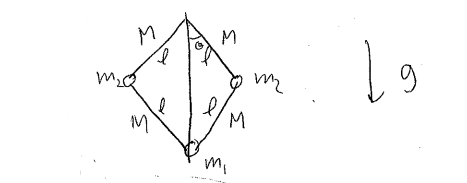
\includegraphics{Problem2}
    \centering
\end{figure}
\begin{enumerate}[label=(\alph*)]
    \item Repeat the three calculations requested in problem 1 from problem set \#2 for this case.
    \item Find the relation between the initial conditions $\theta(0)=\theta_0$ and $\phi(0)=\omega$ such that $\theta$ does not change with time.
    \item Now imagine $m_1$ is given a small upwards impulse. Find the frequency of small oscillations of $\theta$ about $\theta_0$.
\end{enumerate}


\section*{Problem 3}
Model the Earth with its drifiting continental plates as a sphere of mass $M$ with two point masses $m \ll M$ (the ``continents'') on its surface. In a suitable cartesian coordinate system centered at the earth's center and attached to the rotating earth, one point mass lies at $(x,y,z)=R(0,\sin\theta,\cos\theta)$, while the other lies at the mirror image point on the other side of the $x$-$z$ plane, $(x,y,z)=R(0,-\sin\theta,\cos\theta)$ (see figure):
\begin{figure}[H]
    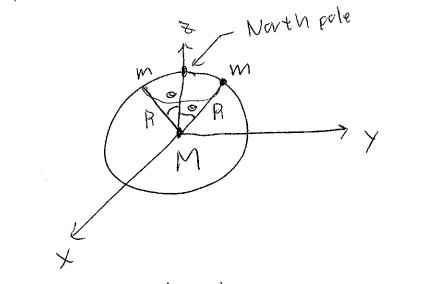
\includegraphics{Problem3}
    \centering
\end{figure}
The radius of the Earth is R.
\begin{enumerate}[label=(\alph*)]
    \item Calculate the moment of inertia tensor of the Earth about the center of the sphere.
    \item Calculate the moment of inertia tensor about the Earth's \underline{center of mass}, and show that, for $m \ll M$, it differs negligibly form that about the center of the sphere. Specifically, show that
    \begin{equation}
        \tilde{I}_\text{cm} - \tilde{I}_\text{center of shpere} \ll \tilde{I}_\text{center of sphere} - \tilde{I}_\text{sphere} \tag{3.1}\label{eq:3.1}
    \end{equation}
    where by $\tilde{I}_\text{sphere}$ I mean the moment of inertia tensor of the sphere of mass $M$ \underline{without} the point masses $m$ about \underline{its} center of mass.
    \item Neglecting the terms you showed to be negligible in part (b), show that, as the continents drift sout (i.e. as $\theta$ increases), at some critical value of $\theta$, roatation about the $z$-axis becomes unstable. Find that critical value of $\theta$.
    \item Assume the continents \underline{are} drifiting southward according to
    \begin{equation}
        \theta(t) = \omega t, \tag{3.2}\label{eq:3.2}
    \end{equation}
    with $\omega \ll \Omega$, where $\Omega$ is the rotation rate of the earth ($\Omega = \frac{2\pi}{1 \text{ day}}$). Find the linearized equations of motion for the angular momentum vector $\vec{L}$ in the Earth's co-rotating frame for rotation nearly (but not exactly) around the $z$-axis, and estimate how long it takes after the instability sets in for $\vec{L}$ to wander an appreciable angle (say, $45^{\circ}$) over the Earth's surface. Assume the inital angle between $\vec{L}$ and $\hat{z}$ is around $10^{-5}$ radians, and take $\frac{m}{M}=10^{-3}$, and $\omega=(10^8 \text{ years})^{-1}$. \\ Hint: to solve a differential equation of the form you're likely to encounter, try a solution of the form \[ y(t) = Ae^{Bt^\alpha}, \] and find the value of $\alpha$ that solves the equation approximately at large times.
\end{enumerate}



\section*{Problem 4}
Three identical masses are connected by indentical springs. Two of the masses slide (need I say `frictionlessly'?) on a straight rigid rod, as shown:
\begin{figure}[H]
    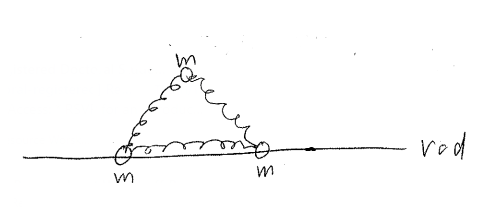
\includegraphics{Problem4}
    \centering
\end{figure}
The equilibrium length of each spring is $l_0$, and their spring cosntant is $k$.
\begin{enumerate}[label=(\alph*)]
    \item Write down the Lagrangian for this system. (NOTE: $l_0 \neq 0$)
    \item Find its fixed points.
    \item Find the eigenfrequencies / growth-decay rates for small motions around these fixed ponts (hint: use symmetry arguments to guess the normal modes). Which fixed points are stable, and which are unstable?
\end{enumerate}

\end{document}